\chapter{总体设计}
\section{软件描述}
%系统包括前台和后台两个部分。

%前台主要功能是:

%后台主要功能是:
系统包括客户端和服务端两个部分。

客户端为用户提供图形界面,用户可以在客户端上登陆账号,搜索添加好友,和好友聊天,参与群聊,发送语音视频消息。

服务端为客户端提供支持,存储用户数据和消息记录,在不同用户间转发聊天消息,提供搜索功能。

\section{处理流程}
\subsection{总体流程}
%此处应当有一个图和对应的描述。

\begin{figure}[h]
	\centering
	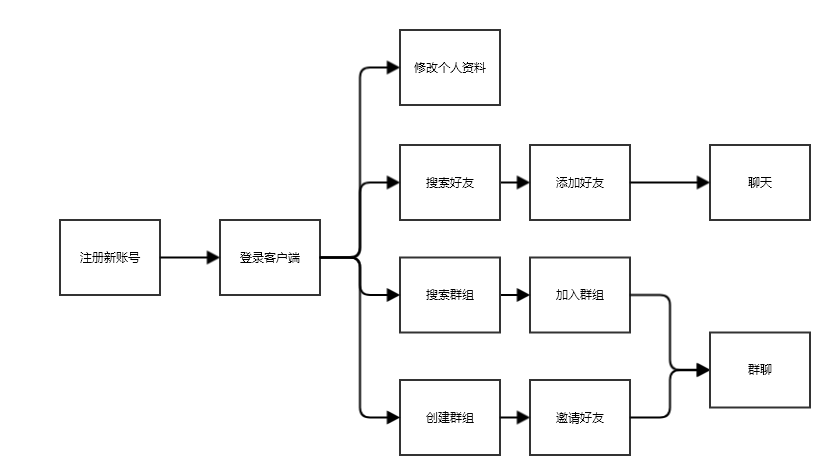
\includegraphics[width=13cm]{base_flowchart}
	\caption{总体流程图} \label{fig:base_flowchart}
\end{figure}

%\subsection{系统基本流程}
%此处应当有一个图和对应的描述。

\subsection{客户端基本流程}
%这只是举个例子,如果没有客户端则不需要此节。
\begin{figure}[h]
	\centering
	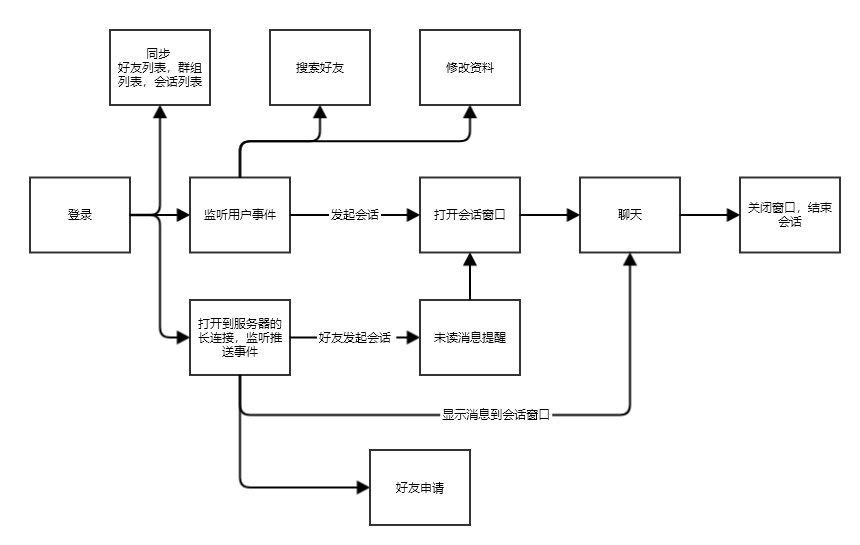
\includegraphics[width=13cm]{client_flowchart}
	\caption{客户端流程图} \label{fig:client_flowchart}
\end{figure}
用户在登陆账号后,客户端会从服务器同步好友,群组和会话信息。并打开一个到服务器的长连接,监听服务器的推送消息。
用户可以点击好友列表或群组列表中的项目启动一个会话窗口,在会话窗口中发送各种消息。
服务器会及时推送消息给客户端,客户端会将消息及时显示到对应的窗口中。
客户端也提供好友搜索,个人资料修改等功能。

\subsection{服务器端基本流程}
%这只是举个例子,如果没有服务器端则不需要此节。
\begin{figure}[h]
	\centering
	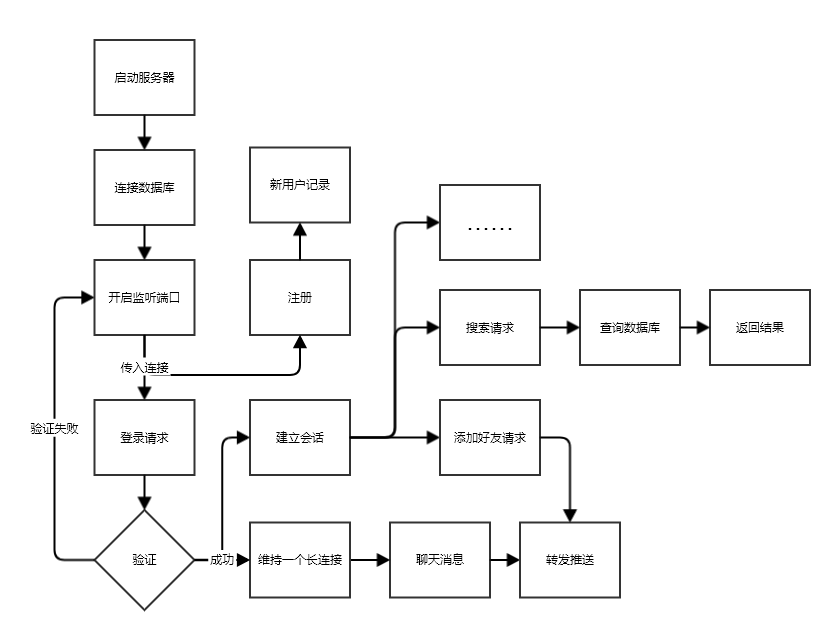
\includegraphics[width=13cm]{server_flowchart}
	\caption{服务端流程图} \label{fig:server_flowchart}
\end{figure}

\subsection{功能1具体流程}
举个例子:交易处理流程

已登录用户在购物车中提交请求交易的 POST 请求,提交的表单中指明了交易中包括的
所有商品、商家、付款信息、收货地址,输入输出处理系统接收到合法请求后,向商品信息
系统请求数据,收到数据以后验证是否正确,然后向订单系统发起生成新订单的请求,订单
系统负责更新商品信息系统、商家信息,通知商家接单,返回订单处理结果输入输出处理系
统,输入输出处理系统依照结果产生 HTML 页面,并返回给用户。

\subsection{功能2具体流程}
此处应当有描述。

\subsection{用户搜索功能具体流程}
%此处应当有一个描述。
\begin{figure}[h]
	\centering
	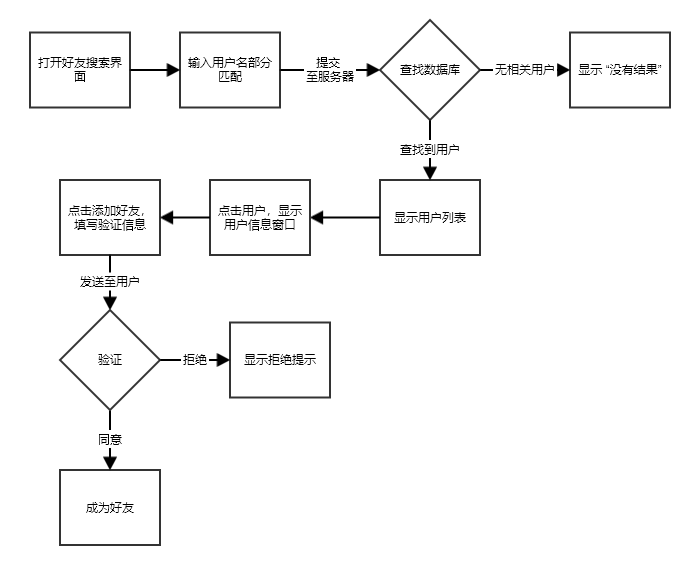
\includegraphics[width=13cm]{search_friend_flowchart}
	\caption{用户搜索功能流程图} \label{fig:search_friend_flowchart}
\end{figure}


\section{功能结构设计}
\subsection{整体结构}
此处应当有一个图和对应的描述。系统如果像微内核那样,划分成核心模块和若干个子系统,此处应当有图示及说明,然后后续几个节应当描述这几个子系统。如果系统像宏内核,那应当说明有哪些紧密联系的模块,并在后续几个节内描述这些模块。

\subsection{用户端结构}
此处应当有一个图和对应的描述。这只是举个例子。可能的内容包括用户端的具体模块、耦合情况等。

\subsection{服务器端结构}
此处应当有一个图和对应的描述。这只是举个例子。

\subsection{后台数据库维护模块结构}
此处应当有一个图和对应的描述。这只是举个例子。



\section{功能需求与程序代码的关系}
[此处指的是不同的需求分配到哪些模块去实现。可按不同的端拆分此表]
\begin{table}[htbp]
\centering
\caption{功能需求与程序代码的关系表} \label{tab:requirement-module}
\begin{tabular}{|c|c|c|c|}
    \hline
    · & 模块1 & 模块2 & 模块3 \\
    \hline
    需求1 & · & Y & · \\
    \hline
    需求2 & · & Y & · \\
    \hline
    需求3 & · & Y & · \\
    \hline
    需求4 & Y & · & · \\
    \hline
    需求5 & · & · & Y \\
    \hline
\end{tabular}
\note{各项功能需求的实现与各个程序模块的分配关系}
\end{table}